%!TEX root = ../dissertation.tex
%
\begin{savequote}[75mm]
Humility has negative impact factor.
\qauthor{Professor Rajibul Kazim Islam}
\end{savequote}

\chapter{Conclusion}
\label{sec:conclusion}

\section{Summary}

In this thesis, I have presented results that discern the behavior of quantum correlations in both equilibrium and non-equilibrium phase transitions. A framework is presented for distinguishing between quantum-thermalizing and many-body-localized phases by observing the dynamics of such correlations in a Bose-Hubbard system. Additionally, the observations of spatial correlations persisting to high orders in the critical regime demonstrates  the value of using a quantum gas microscope to observe highly correlated, novel quantum phenomena. 
%n a quantum gas microscope allow for experimental observation 

For the case of the equilibrium quantum phase transition of the transverse Ising model, we can directly measure the order parameter as we cross the phase transition and the effect of boundary conditions on the ground state. We additionally measure an increase of entanglement entropy near the critical point that qualitatively aligns with the phenomenology of traditional phase transition behavior\cite{Sachdev2011}. In the case of the superfluid-to-Mott-insulator transition, we directly measure the entropy via the second-order R\'enyi entropy and verify that it arises from modal entanglement of the many-body quantum state\cite{Islam2015}.

In the context of a non-equilibrium phase transition, we directly measure that, after a quantum quench, an isolated quantum many-body system rapidly approaches local agreement with predictions given by a statistical ensemble. The entanglement entropy measured via the R\'enyi entropy in this system is analogous to the thermal entropy expected for a truly thermal system. These observations agree with the predictions of the eigenstate thermalization hypothesis that isolated quantum systems locally resemble classical ensembles\cite{Kaufman2016}. However, the robust exception to this behavior is generated by the application of on-site disorder potentials that prevent the system from thermalizing and qualitatively changes its entanglement dynamics. We observe a logarithmically slow growth of entanglement in such a many-body-localized system and measure the subsystem-size scaling behavior of entanglement in both the thermalizing and localized phases\cite{Lukin2019}.

We additionally explore the transition between these two non-equilibrium phases. We find a system-size dependence in the thermalization of these isolated quantum systems that identifies their critical behavior. In the two extremes of low and high disorder, we find system-size independent thermalization and localization, respectively. Near the critical point of the transition we observe an increase in correlations that persists up to high orders. Additionally, these correlations are highly-structured and suggest that it is not all sites in the system that contribute to this critical thermalization, but it is a sparse-resonant network of sites that leads the system towards equilibration. These results lay the foundation for experimentally studying the critical behavior of non-equilibrium phase transitions and whether many of the same concepts from traditional equilibrium phase transitions framework can be applied to these systems\cite{Rispoli2018}.

\section{Outlook}

The results in this thesis have demonstrated novel measurement techniques, long coherence times, precise system-size scalability, and framework for understanding the growth of correlations in a non-equilibrium system. However, many open questions about the thermal-to-MBL phase transition still remain. Some of these questions can be straight-forwardly implemented in our system through several new studies:

%\subsection{Driven Systems ?}
%
%The lack of thermalization in a many-body-localized system originates from the formation of an extensive number of conserved quantities that prevent the redistribution of energy in the system that is required by thermalization. Periodically driven systems are not time-independent and add energy into the system as a function of time. However, since thermalization is not allowed within the system, heating only exists among local degrees of freedom (cite driving papers). It has also been shown that driving the system will in some cases actually induce localization and an MBL phase may appear as a function of driving strength (cite arXiv:1702.06208). The techniques for probing such physics have already been shown for this apparatus and could be easily be applied to the variety of proposals given\cite{Tai2017}. The difficulty of such experiments however revolving around a sufficiently large separation of energy scales and the effect of excitations to higher bands in such a physically driven system.

\subsection{Localization in different disorder distributions}

For all the experiments involving localization in this thesis, the on-site potential offsets used for localization of the many-body states were drawn form a quasi-periodic distribution. This effectively realizes many-body localization in the interacting Aubry-Andr\'e model. While localization is not unique to this distribution, it has been predicted by numerical studies that different disorder distributions may lead to different universality classes of such a transition\cite{Khemani2017a,Zhang2018}. The DMD used for applying the on-site potentials in the presented experiments can be easily adjusted to generate different potential distributions (e.g. binary disorder, uniform-random disorder, etc.). Studying the critical behavior of this system in different potential distributions will help shed light on the presence of universality in these non-equilibrium systems \cite{Khemani2017a,Zhang2018,Setiawan2017}.

% with a periodicity that is incommensurate with the Bose-Hubbard lattice

\subsection{Mechanisms for thermalization}

Additionally, the microscopic mechanism that leads to thermalization in different disorder distributions may qualitatively differ. The microscopic resolution of correlations in these systems afforded by the quantum gas microscope would allow for an extended study of the microscopic picture for how such systems thermalize \cite{Potter2015,Vosk2015,Zhang2018,Roeck2017,Luitz2017,Ponte2017}. 

\begin{figure}[t!]
		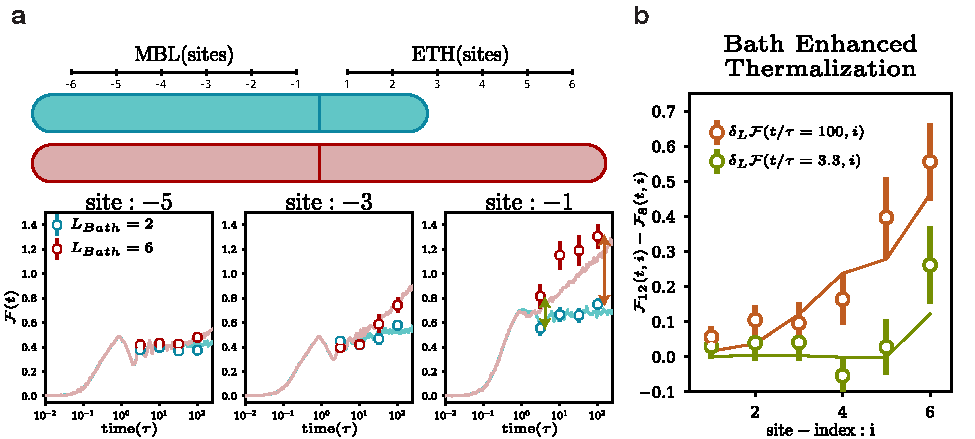
\includegraphics[width=\columnwidth]{figures/ch7/bath_thermal/BathSSFig.pdf} 
		\caption{\textbf{Thermalization from bath. a)} The thermalization of a $6$-site MBL system due to local contact with a thermal bath is compared for two different bath sizes : a $2$-site bath (blue) and a $6$-site bath (red). The site indices reflect there distance from the left-most end of the MBL system: $i=6$ is the first MBL site closets to the bath, $i=1$ is the MBL site furthest from the bath. We find that only the larger bath size causes a slow growth of the on-site fluctuations which typically herald the agreement with a thermal ensemble. \textbf{b)} The difference between the on-site fluctuations of the two different bath sizes are compared site-by-site for two different times: $t=3\tau$ (green) and $t=100\tau$ (orange). The green line (early time) demonstrates a near agreement at early times between the two different system sizes, while the orange line (late time) shows a significant, site dependent thermalization away from the bath. The solid lines are calculated from exact numerics. The error bars are the s.e.m.}
		\label{fig:bath_sz}	
\end{figure}

As a preliminary study of a particular mechanism, we experimentally implement the effect of anomalously low-disorder regions that would exist in truly random on-site disorder. It is believed that such regions will behave like thermal systems and create a so-called ``avalanche" that drives the remaining system towards thermalization\cite{Roeck2017,Luitz2017}. To probe such a mechanism, we measured the local number fluctuations in a many-body-localized system that is in contact with a variable-size ergodic grain. The many-body-localized system experiences quasi-periodic disorder and in a system with no bath remains localized for long times. We observe that in the two studied cases, a bath size of $2$-sites and a bath size of $6$-sites, the smaller system  remains localized for all measured times while the system with the larger bath size shows a slow relaxation towards thermal equilibrium with a spatial dependence that mimics the proposed ``avalanche" mechanism.

 \begin{figure}[t!]
		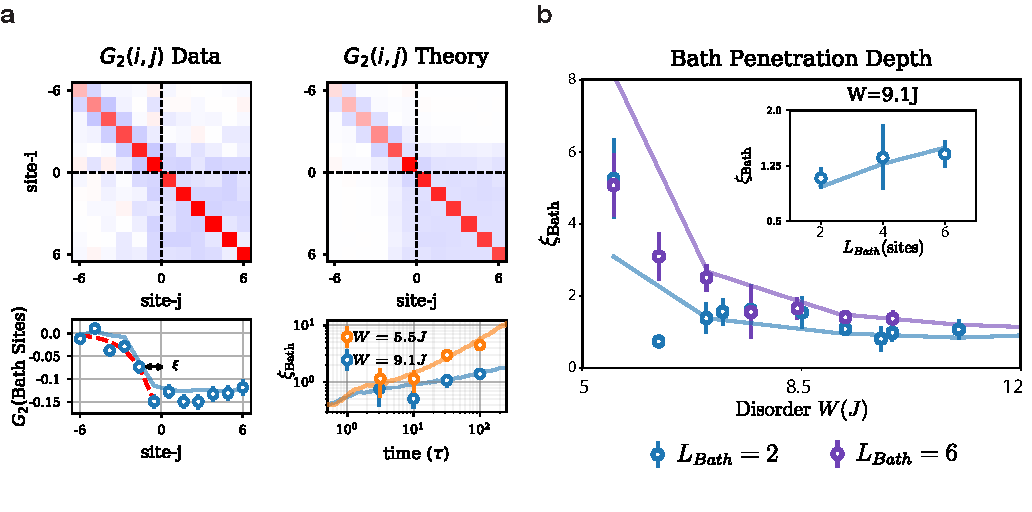
\includegraphics[width=\columnwidth]{figures/ch7/bathfig.pdf} 
		\caption{\textbf{Penetration depth. a)} We directly probe the bath penetration depth by averaging over the two-point correlations from bath sites to MBL sites ($G^{(2)}_c(i,j)$). The extracted correlation length (bottom left) is then calculated by the first moment and plotted as a function of time for a critical system (orange, $W=5.5J$) and an MBL system (blue, $W=9.1J$). \textbf{b)}  We then compare the extracted localization length$\xi_{Bath}$ at long times ($t=100\tau$) for both the $2$-site bath system (blue) and the $6$-site bath system (orange) as a function of disorder. We then compare the this length scale as a function of total bath size for the MBL disorder regime (inset).}
		\label{fig:bath_depth}	
\end{figure}

The enhanced thermalization in the larger bath-size system grows as a function of distance away from the bath-MBL interface. This is consistent with the avalanche process acting as a bath that incorporates nearby non-thermal systems that then enhance the bandwidth of thermalizing bubble that then spatially drives the system as a whole towards equilibrium. This can be visualized by comparing the penetration depth of the bath into the localized system where we see the larger system has a penetration depth that grows with time -- unlike the smaller bath system (as seen in Fig~\ref{fig:bath_depth}).

These preliminary studies suggest that the avalanche-like process is likely a viable mechanism for thermalizing disordered systems. This mechanism seems like a conceptually natural method for systems with random disorder to eventually thermalize since sufficiently large systems will contain large ergodic grains known as Griffiths regions. In this study, this hybrid system of a quasi-periodic disordered system in physical contact with an ergodic grain is similar to adding such a non-disordered Griffiths region in a randomly disordered system.\footnote{Griffiths regions often refer to a rare region of anomalously large disorder that acts like a bottle neck for hindering the spread of information in a system. These regions will exist in large random-disorder systems due the stochastic likelihood of sampling several significantly different on-site potential values that are also neighboring in space. However, in this case I am referring to the opposite likelihood of sampling very similar values for on-site potential values for neighboring sites in space that would allow for anomalously low disorder regions that would look locally thermal and potentially act as a bath for the remaining system.}  There is an additional caveat to this physical implementation that relates to a suggestion that the critical behavior for quasi-periodic and random potentials might be of different universality classes\cite{Khemani2017a,Zhang2018}, in which case it is unclear whether the observed behavior will quantitatively agree with either. This emphasizes the importance of further studies of thermalization in such disordered systems by engineering the presence of ergodic grains and also realizing multiple disorder distribution classes.


%\subsection{Additional degrees of freedom}
%
%Other open questions about many-body localization relate to which available degrees of freedom become localized as emergent degrees of freedom from the application of disorder. In particular, a proposal for studying a multi-spin component Bose-Hubbard system would also lose initial information its initial state spin pattern. Since exchanging any two spins would result in nearly the same energy of the system even though particle transport, where the spins may act as a distinguishing label for the particles, remain localized by the disorder. (cite whichever paper)

\subsection{Localization in Fock space}

One of the first approaches taken to solve the MBL problem was to cast it back to a single-particle problem by looking at the system in Fock space \cite{Altshuler1997,Alet2018}. This then makes every Fock state a single node in a large, multi-dimensional space where the on-site disorder for each node both depends upon the interaction energy $U$ and the experienced on-site disorder $W_i$. This is shown schematically in Fig.~\ref{fig:hamD}.

\begin{figure}[t!]
		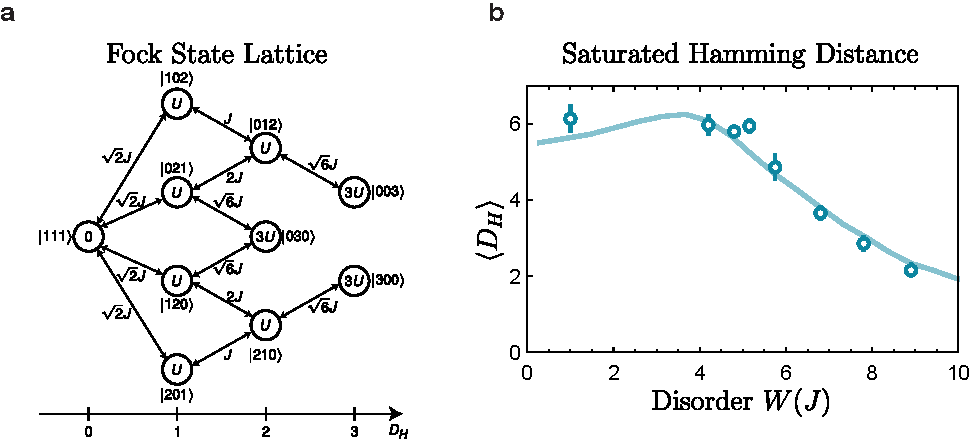
\includegraphics[width=\columnwidth]{figures/ch7/hamming_dist_fig.pdf} 
		\caption{\textbf{Hamming distance $(D_H)$. a)} A schematic of the mapping to a Fock state lattice of $3$-sites at unity filling. Each node in this lattice represents a given Fock state. The nodes have an on-site energy determined by their interaction and potential offsets. They are still coupled by the tunneling matrix elements $J$. This effectively casts the many-body problem into a multi-dimensional, single-particle problem. The number of hops away from the initial state are encoded along the $x$-axis and are labeled as the Bose-Hubbard version of the Hamming distance $(D_H)$. \textbf{b)} The Hamming distance is measured at late times  $(t=100\tau)$ and plotted as a function of disorder strength $W$ for an $8$-site Bose-Hubbard system after the  protocol defined in \S \ref{sec:ch5}.  The decrease in final Hamming distance as a function of $W$ indicates  localization in Fock space.}
		\label{fig:hamD}	
\end{figure}

Since we have direct access to the many-body state in the Fock basis at the end of each experimental run, we can experimentally verify the localization of the system in Fock space. In some preliminary experiments, we quantify the localization of the state through the Fock-space Hamming distance. Traditionally, the Hamming distance is a concept from computer science that defines how many bit flips away a string of bits is from its original configuration. This is modified to the case of bosons hopping in a lattice by determining the minimum number of hopping events a state has moved away from its initial state ($D_H$). In Fig.~\ref{fig:hamDmoments} we show the evolution of the first and second moments of $D_H$ in the thermalizing, MBL, and critical regimes of disorder as a function of time. This preliminary study seems to show a persistence of evolution in the diffusion of the system in Fock space while the first moment remains stationary at a finite value.

\begin{figure}[t!]
		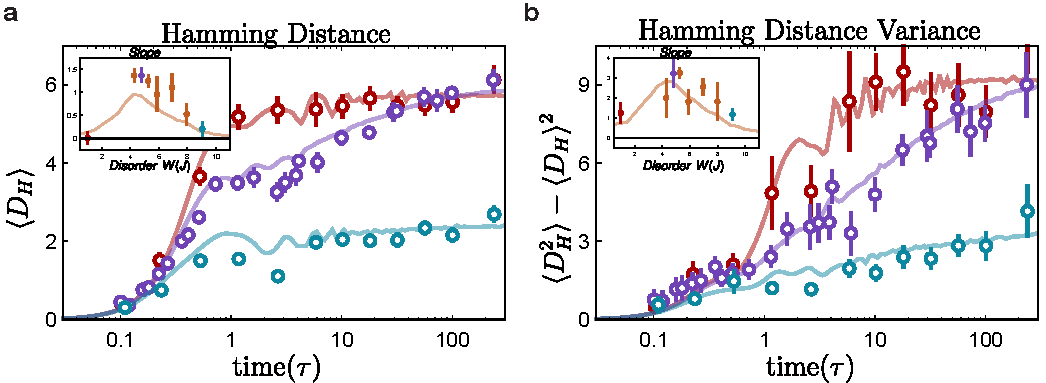
\includegraphics[width=\columnwidth]{figures/ch7/hamming_dist_slopes_fig.pdf} 
		\caption{\textbf{First and second moments of Hamming distance. a)} The first moment of the Hamming distance,$\langle D_H \rangle$ is plotted as a function of time for the thermalizing (red), critical (purple), and MBL (blue) regimes. The slopes of these growth curves are extracted from a semi-log plot for $L/2 \tau < t \leq 100 \tau$ and shown in the inset as a function of disorder. \textbf{b)}  The second moment of the Hamming distance,$\langle \left ( D_H - \langle D_H \rangle  \right )^2 \rangle$ is plotted as a function of time for the thermalizing (red), critical (purple), and MBL (blue) regimes. The slopes of these growth curves are extracted from a semi-log plot for $L/2 \tau < t \leq 100 \tau$ and shown in the inset as a function of disorder.}
		\label{fig:hamDmoments}	
\end{figure}

However, since the original intention was to look at whether the system localizes in Fock space, one needs to normalize this system by the density of states at a given Hamming distance. This approach is only marginally more complicated than in real space since the dimensionality, or connectivity, of the system changes as a function of a given node. This density of states as a function of $D_H$, as well as the measured, long-time probability distributions have not been normalized. Note that when normalized by the density of states, all quench experiments will appear to be localized to some finite value. This is partially due to the cost in energy associated with multiple occupancies in Fock space, which appears as an effective trapping potential in this basis. Therefore, all finite energy density quench experiments will likely have a finite localization length less than the total system size.

%
%\subsection{Multifractality}
%
%WHAT ABOUT DIFFERENT INITIAL STATES AND DIFFERENT INITIAL ENERGIES?
%
%PROTECTION OF SYMMETRY AND PHASE TRANSITIONS AMONG MANY EIGENSTATES, CITE HUSE

